\documentclass[twoside]{book}

% Packages required by doxygen
\usepackage{fixltx2e}
\usepackage{calc}
\usepackage{doxygen}
\usepackage[export]{adjustbox} % also loads graphicx
\usepackage{graphicx}
\usepackage[utf8]{inputenc}
\usepackage{makeidx}
\usepackage{multicol}
\usepackage{multirow}
\PassOptionsToPackage{warn}{textcomp}
\usepackage{textcomp}
\usepackage[nointegrals]{wasysym}
\usepackage[table]{xcolor}

% NLS support packages
\usepackage[T2A]{fontenc}
\usepackage[russian]{babel}

% Font selection
\usepackage[T1]{fontenc}
\usepackage[scaled=.90]{helvet}
\usepackage{courier}
\usepackage{amssymb}
\usepackage{sectsty}
\renewcommand{\familydefault}{\sfdefault}
\allsectionsfont{%
  \fontseries{bc}\selectfont%
  \color{darkgray}%
}
\renewcommand{\DoxyLabelFont}{%
  \fontseries{bc}\selectfont%
  \color{darkgray}%
}
\newcommand{\+}{\discretionary{\mbox{\scriptsize$\hookleftarrow$}}{}{}}

% Page & text layout
\usepackage{geometry}
\geometry{%
  a4paper,%
  top=2.5cm,%
  bottom=2.5cm,%
  left=2.5cm,%
  right=2.5cm%
}
\tolerance=750
\hfuzz=15pt
\hbadness=750
\setlength{\emergencystretch}{15pt}
\setlength{\parindent}{0cm}
\setlength{\parskip}{3ex plus 2ex minus 2ex}
\makeatletter
\renewcommand{\paragraph}{%
  \@startsection{paragraph}{4}{0ex}{-1.0ex}{1.0ex}{%
    \normalfont\normalsize\bfseries\SS@parafont%
  }%
}
\renewcommand{\subparagraph}{%
  \@startsection{subparagraph}{5}{0ex}{-1.0ex}{1.0ex}{%
    \normalfont\normalsize\bfseries\SS@subparafont%
  }%
}
\makeatother

% Headers & footers
\usepackage{fancyhdr}
\pagestyle{fancyplain}
\fancyhead[LE]{\fancyplain{}{\bfseries\thepage}}
\fancyhead[CE]{\fancyplain{}{}}
\fancyhead[RE]{\fancyplain{}{\bfseries\leftmark}}
\fancyhead[LO]{\fancyplain{}{\bfseries\rightmark}}
\fancyhead[CO]{\fancyplain{}{}}
\fancyhead[RO]{\fancyplain{}{\bfseries\thepage}}
\fancyfoot[LE]{\fancyplain{}{}}
\fancyfoot[CE]{\fancyplain{}{}}
\fancyfoot[RE]{\fancyplain{}{\bfseries\scriptsize Создано системой Doxygen }}
\fancyfoot[LO]{\fancyplain{}{\bfseries\scriptsize Создано системой Doxygen }}
\fancyfoot[CO]{\fancyplain{}{}}
\fancyfoot[RO]{\fancyplain{}{}}
\renewcommand{\footrulewidth}{0.4pt}
\renewcommand{\chaptermark}[1]{%
  \markboth{#1}{}%
}
\renewcommand{\sectionmark}[1]{%
  \markright{\thesection\ #1}%
}

% Indices & bibliography
\usepackage{natbib}
\usepackage[titles]{tocloft}
\setcounter{tocdepth}{3}
\setcounter{secnumdepth}{5}
\makeindex

% Hyperlinks (required, but should be loaded last)
\usepackage{ifpdf}
\ifpdf
  \usepackage[pdftex,pagebackref=true]{hyperref}
\else
  \usepackage[ps2pdf,pagebackref=true]{hyperref}
\fi
\hypersetup{%
  colorlinks=true,%
  linkcolor=blue,%
  citecolor=blue,%
  unicode%
}

% Custom commands
\newcommand{\clearemptydoublepage}{%
  \newpage{\pagestyle{empty}\cleardoublepage}%
}

\usepackage{caption}
\captionsetup{labelsep=space,justification=centering,font={bf},singlelinecheck=off,skip=4pt,position=top}

%===== C O N T E N T S =====

\begin{document}

% Titlepage & ToC
\hypersetup{pageanchor=false,
             bookmarksnumbered=true,
             pdfencoding=unicode
            }
\pagenumbering{alph}
\begin{titlepage}
\vspace*{7cm}
\begin{center}%
{\Large T\+OB }\\
\vspace*{1cm}
{\large Создано системой Doxygen 1.8.13}\\
\end{center}
\end{titlepage}
\clearemptydoublepage
\pagenumbering{roman}
\tableofcontents
\clearemptydoublepage
\pagenumbering{arabic}
\hypersetup{pageanchor=true}

%--- Begin generated contents ---
\chapter{Алфавитный указатель пространств имен}
\section{Пространства имен}
Полный список пространств имен.\begin{DoxyCompactList}
\item\contentsline{section}{\hyperlink{namespaceavailableurl}{availableurl} }{\pageref{namespaceavailableurl}}{}
\item\contentsline{section}{\hyperlink{namespacedownloadxml}{downloadxml} }{\pageref{namespacedownloadxml}}{}
\item\contentsline{section}{\hyperlink{namespaceextractip}{extractip} }{\pageref{namespaceextractip}}{}
\item\contentsline{section}{\hyperlink{namespacerecognizeip}{recognizeip} }{\pageref{namespacerecognizeip}}{}
\end{DoxyCompactList}

\chapter{Список файлов}
\section{Файлы}
Полный список файлов.\begin{DoxyCompactList}
\item\contentsline{section}{\hyperlink{availableurl_8py}{availableurl.\+py} }{\pageref{availableurl_8py}}{}
\item\contentsline{section}{\hyperlink{downloadxml_8py}{downloadxml.\+py} }{\pageref{downloadxml_8py}}{}
\item\contentsline{section}{\hyperlink{extractip_8py}{extractip.\+py} }{\pageref{extractip_8py}}{}
\item\contentsline{section}{\hyperlink{recognizeip_8py}{recognizeip.\+py} }{\pageref{recognizeip_8py}}{}
\end{DoxyCompactList}

\chapter{Пространства имен}
\hypertarget{namespaceavailableurl}{}\section{Пространство имен availableurl}
\label{namespaceavailableurl}\index{availableurl@{availableurl}}
\subsection*{Функции}
\begin{DoxyCompactItemize}
\item 
def \hyperlink{namespaceavailableurl_a25d6c72ce2cd54a5490720f1319c68dc}{logger} ()
\begin{DoxyCompactList}\small\item\em Запуск логгера. \end{DoxyCompactList}\item 
def \hyperlink{namespaceavailableurl_aff3d4545f3483782a407aab7859602f4}{Access} ()
\begin{DoxyCompactList}\small\item\em Проверка доступности U\+R\+L-\/адресов. \end{DoxyCompactList}\item 
def \hyperlink{namespaceavailableurl_a9bdd46562a5ef06276fceee5109958e7}{main} ()
\end{DoxyCompactItemize}
\subsection*{Переменные}
\begin{DoxyCompactItemize}
\item 
string \hyperlink{namespaceavailableurl_a37fb41a94b1d571e29110ace71a6779b}{dbhost} = \textquotesingle{}localhost\textquotesingle{}
\item 
string \hyperlink{namespaceavailableurl_a390f7a9e2e87f1ef981f38c17606925a}{dbport} = \textquotesingle{}5432\textquotesingle{}
\item 
string \hyperlink{namespaceavailableurl_a7aad22fecf6c516bded3d3c0a571bd40}{dbuser} = \textquotesingle{}postgres\textquotesingle{}
\item 
string \hyperlink{namespaceavailableurl_a213229dedd788b05a4d417a6e54d5662}{dbpass} = \textquotesingle{}1234\textquotesingle{}
\item 
string \hyperlink{namespaceavailableurl_ac13da61208e787ad038413b3779bf437}{dbname} = \textquotesingle{}project\+\_\+0\textquotesingle{}
\end{DoxyCompactItemize}


\subsection{Функции}
\mbox{\Hypertarget{namespaceavailableurl_aff3d4545f3483782a407aab7859602f4}\label{namespaceavailableurl_aff3d4545f3483782a407aab7859602f4}} 
\index{availableurl@{availableurl}!Access@{Access}}
\index{Access@{Access}!availableurl@{availableurl}}
\subsubsection{\texorpdfstring{Access()}{Access()}}
{\footnotesize\ttfamily def availableurl.\+Access (\begin{DoxyParamCaption}{ }\end{DoxyParamCaption})}



Проверка доступности U\+R\+L-\/адресов. 



См. определение в файле availableurl.\+py строка 47

Граф вызова функции\+:\nopagebreak
\begin{figure}[H]
\begin{center}
\leavevmode
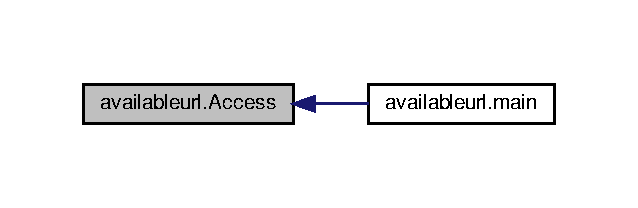
\includegraphics[width=306pt]{namespaceavailableurl_aff3d4545f3483782a407aab7859602f4_icgraph}
\end{center}
\end{figure}
\mbox{\Hypertarget{namespaceavailableurl_a25d6c72ce2cd54a5490720f1319c68dc}\label{namespaceavailableurl_a25d6c72ce2cd54a5490720f1319c68dc}} 
\index{availableurl@{availableurl}!logger@{logger}}
\index{logger@{logger}!availableurl@{availableurl}}
\subsubsection{\texorpdfstring{logger()}{logger()}}
{\footnotesize\ttfamily def availableurl.\+logger (\begin{DoxyParamCaption}{ }\end{DoxyParamCaption})}



Запуск логгера. 



См. определение в файле availableurl.\+py строка 17

Граф вызова функции\+:\nopagebreak
\begin{figure}[H]
\begin{center}
\leavevmode
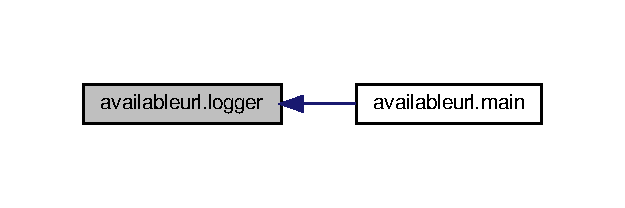
\includegraphics[width=300pt]{namespaceavailableurl_a25d6c72ce2cd54a5490720f1319c68dc_icgraph}
\end{center}
\end{figure}
\mbox{\Hypertarget{namespaceavailableurl_a9bdd46562a5ef06276fceee5109958e7}\label{namespaceavailableurl_a9bdd46562a5ef06276fceee5109958e7}} 
\index{availableurl@{availableurl}!main@{main}}
\index{main@{main}!availableurl@{availableurl}}
\subsubsection{\texorpdfstring{main()}{main()}}
{\footnotesize\ttfamily def availableurl.\+main (\begin{DoxyParamCaption}{ }\end{DoxyParamCaption})}



См. определение в файле availableurl.\+py строка 60

Граф вызовов\+:\nopagebreak
\begin{figure}[H]
\begin{center}
\leavevmode
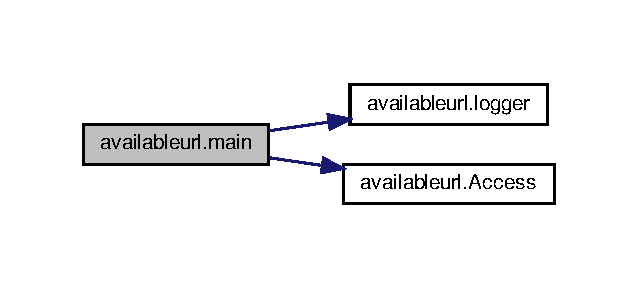
\includegraphics[width=306pt]{namespaceavailableurl_a9bdd46562a5ef06276fceee5109958e7_cgraph}
\end{center}
\end{figure}


\subsection{Переменные}
\mbox{\Hypertarget{namespaceavailableurl_a37fb41a94b1d571e29110ace71a6779b}\label{namespaceavailableurl_a37fb41a94b1d571e29110ace71a6779b}} 
\index{availableurl@{availableurl}!dbhost@{dbhost}}
\index{dbhost@{dbhost}!availableurl@{availableurl}}
\subsubsection{\texorpdfstring{dbhost}{dbhost}}
{\footnotesize\ttfamily string availableurl.\+dbhost = \textquotesingle{}localhost\textquotesingle{}}



См. определение в файле availableurl.\+py строка 7

\mbox{\Hypertarget{namespaceavailableurl_ac13da61208e787ad038413b3779bf437}\label{namespaceavailableurl_ac13da61208e787ad038413b3779bf437}} 
\index{availableurl@{availableurl}!dbname@{dbname}}
\index{dbname@{dbname}!availableurl@{availableurl}}
\subsubsection{\texorpdfstring{dbname}{dbname}}
{\footnotesize\ttfamily string availableurl.\+dbname = \textquotesingle{}project\+\_\+0\textquotesingle{}}



См. определение в файле availableurl.\+py строка 11

\mbox{\Hypertarget{namespaceavailableurl_a213229dedd788b05a4d417a6e54d5662}\label{namespaceavailableurl_a213229dedd788b05a4d417a6e54d5662}} 
\index{availableurl@{availableurl}!dbpass@{dbpass}}
\index{dbpass@{dbpass}!availableurl@{availableurl}}
\subsubsection{\texorpdfstring{dbpass}{dbpass}}
{\footnotesize\ttfamily string availableurl.\+dbpass = \textquotesingle{}1234\textquotesingle{}}



См. определение в файле availableurl.\+py строка 10

\mbox{\Hypertarget{namespaceavailableurl_a390f7a9e2e87f1ef981f38c17606925a}\label{namespaceavailableurl_a390f7a9e2e87f1ef981f38c17606925a}} 
\index{availableurl@{availableurl}!dbport@{dbport}}
\index{dbport@{dbport}!availableurl@{availableurl}}
\subsubsection{\texorpdfstring{dbport}{dbport}}
{\footnotesize\ttfamily string availableurl.\+dbport = \textquotesingle{}5432\textquotesingle{}}



См. определение в файле availableurl.\+py строка 8

\mbox{\Hypertarget{namespaceavailableurl_a7aad22fecf6c516bded3d3c0a571bd40}\label{namespaceavailableurl_a7aad22fecf6c516bded3d3c0a571bd40}} 
\index{availableurl@{availableurl}!dbuser@{dbuser}}
\index{dbuser@{dbuser}!availableurl@{availableurl}}
\subsubsection{\texorpdfstring{dbuser}{dbuser}}
{\footnotesize\ttfamily string availableurl.\+dbuser = \textquotesingle{}postgres\textquotesingle{}}



См. определение в файле availableurl.\+py строка 9


\hypertarget{namespacedownloadxml}{}\section{Пространство имен downloadxml}
\label{namespacedownloadxml}\index{downloadxml@{downloadxml}}
\subsection*{Функции}
\begin{DoxyCompactItemize}
\item 
def \hyperlink{namespacedownloadxml_abc3f6c8d51f9a903bb8504a7ad9ad2de}{logger} ()
\begin{DoxyCompactList}\small\item\em Запуск логгера. \end{DoxyCompactList}\item 
def \hyperlink{namespacedownloadxml_a7f19cfa93073885f474cf6a2a3f25e7f}{Sender} (file)
\begin{DoxyCompactList}\small\item\em Перемещение файлов и отправка в базу данных. \end{DoxyCompactList}\item 
def \hyperlink{namespacedownloadxml_ae15b4d4f7f282d34e48e03a2452741d6}{File\+List} ()
\begin{DoxyCompactList}\small\item\em Получение списка xml-\/файлов. \end{DoxyCompactList}\item 
def \hyperlink{namespacedownloadxml_a801fc32a7254a9319cb06fb65fb757e9}{Download} ()
\begin{DoxyCompactList}\small\item\em Скачивание списоков угроз. \end{DoxyCompactList}\item 
def \hyperlink{namespacedownloadxml_ac0d6bf93a1be6263a0b94ef18bb9c459}{main} ()
\end{DoxyCompactItemize}
\subsection*{Переменные}
\begin{DoxyCompactItemize}
\item 
string \hyperlink{namespacedownloadxml_a75453296d7099653f232694ed5824b3f}{dbhost} = \textquotesingle{}localhost\textquotesingle{}
\item 
string \hyperlink{namespacedownloadxml_a32bdf9e8d022578666b5b9993714c4ef}{dbport} = \textquotesingle{}5432\textquotesingle{}
\item 
string \hyperlink{namespacedownloadxml_ae0187d21bda573cccc7c253c38ac9494}{dbuser} = \textquotesingle{}postgres\textquotesingle{}
\item 
string \hyperlink{namespacedownloadxml_af527b05230cf500f27f1a899351d60af}{dbpass} = \textquotesingle{}1234\textquotesingle{}
\item 
string \hyperlink{namespacedownloadxml_ab0bd228b1313bba2e1fe1caa883e5b6c}{dbname} = \textquotesingle{}project\+\_\+0\textquotesingle{}
\item 
string \hyperlink{namespacedownloadxml_ac658e5e8b5ee862abc49621fce2f449a}{Save\+Dir} = \textquotesingle{}../IN/C\+IC/\textquotesingle{}
\item 
string \hyperlink{namespacedownloadxml_ae93409e2d65411e5e0c56c338629a095}{Move\+Dir} = \textquotesingle{}../O\+UT/C\+IC/\textquotesingle{}
\item 
list \hyperlink{namespacedownloadxml_a89324d9cb91e8b04605a33cb8a959ac9}{urls} = \mbox{[}\textquotesingle{}http\+://bdu.\+fstec.\+ru/documents/files/vulxml.\+zip\textquotesingle{}, \textquotesingle{}http\+://cve.\+mitre.\+org/data/downloads/allitems.\+xml.\+gz\textquotesingle{}\mbox{]}
\item 
int \hyperlink{namespacedownloadxml_a664dcd7a63115699604c60cc1c94b6db}{Sleep} = 86400
\end{DoxyCompactItemize}


\subsection{Функции}
\mbox{\Hypertarget{namespacedownloadxml_a801fc32a7254a9319cb06fb65fb757e9}\label{namespacedownloadxml_a801fc32a7254a9319cb06fb65fb757e9}} 
\index{downloadxml@{downloadxml}!Download@{Download}}
\index{Download@{Download}!downloadxml@{downloadxml}}
\subsubsection{\texorpdfstring{Download()}{Download()}}
{\footnotesize\ttfamily def downloadxml.\+Download (\begin{DoxyParamCaption}{ }\end{DoxyParamCaption})}



Скачивание списоков угроз. 

Распаковка архивов. 

См. определение в файле downloadxml.\+py строка 83

Граф вызовов\+:\nopagebreak
\begin{figure}[H]
\begin{center}
\leavevmode
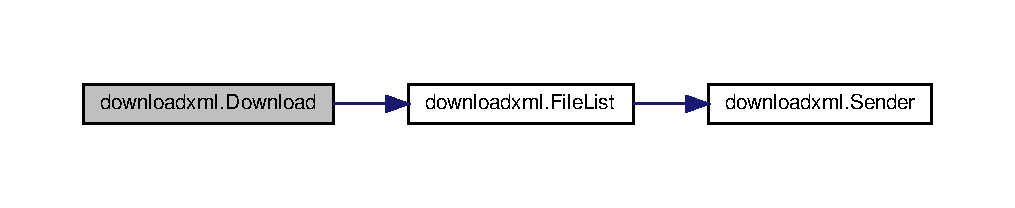
\includegraphics[width=350pt]{namespacedownloadxml_a801fc32a7254a9319cb06fb65fb757e9_cgraph}
\end{center}
\end{figure}
Граф вызова функции\+:\nopagebreak
\begin{figure}[H]
\begin{center}
\leavevmode
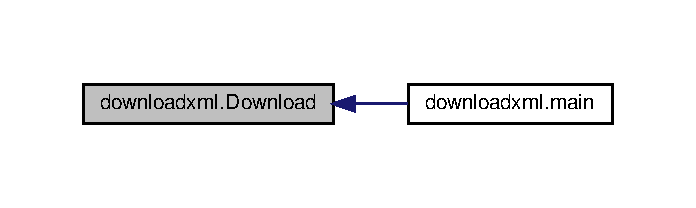
\includegraphics[width=334pt]{namespacedownloadxml_a801fc32a7254a9319cb06fb65fb757e9_icgraph}
\end{center}
\end{figure}
\mbox{\Hypertarget{namespacedownloadxml_ae15b4d4f7f282d34e48e03a2452741d6}\label{namespacedownloadxml_ae15b4d4f7f282d34e48e03a2452741d6}} 
\index{downloadxml@{downloadxml}!File\+List@{File\+List}}
\index{File\+List@{File\+List}!downloadxml@{downloadxml}}
\subsubsection{\texorpdfstring{File\+List()}{FileList()}}
{\footnotesize\ttfamily def downloadxml.\+File\+List (\begin{DoxyParamCaption}{ }\end{DoxyParamCaption})}



Получение списка xml-\/файлов. 



См. определение в файле downloadxml.\+py строка 71

Граф вызовов\+:\nopagebreak
\begin{figure}[H]
\begin{center}
\leavevmode
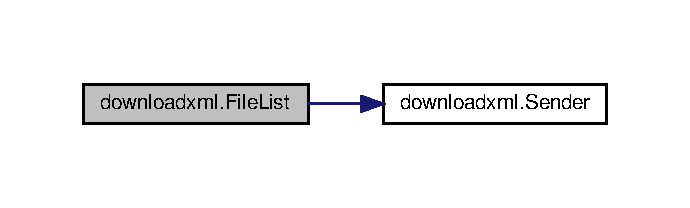
\includegraphics[width=331pt]{namespacedownloadxml_ae15b4d4f7f282d34e48e03a2452741d6_cgraph}
\end{center}
\end{figure}
Граф вызова функции\+:\nopagebreak
\begin{figure}[H]
\begin{center}
\leavevmode
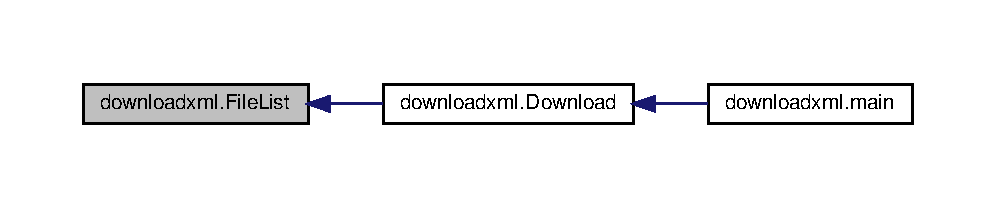
\includegraphics[width=350pt]{namespacedownloadxml_ae15b4d4f7f282d34e48e03a2452741d6_icgraph}
\end{center}
\end{figure}
\mbox{\Hypertarget{namespacedownloadxml_abc3f6c8d51f9a903bb8504a7ad9ad2de}\label{namespacedownloadxml_abc3f6c8d51f9a903bb8504a7ad9ad2de}} 
\index{downloadxml@{downloadxml}!logger@{logger}}
\index{logger@{logger}!downloadxml@{downloadxml}}
\subsubsection{\texorpdfstring{logger()}{logger()}}
{\footnotesize\ttfamily def downloadxml.\+logger (\begin{DoxyParamCaption}{ }\end{DoxyParamCaption})}



Запуск логгера. 



См. определение в файле downloadxml.\+py строка 27

Граф вызова функции\+:\nopagebreak
\begin{figure}[H]
\begin{center}
\leavevmode
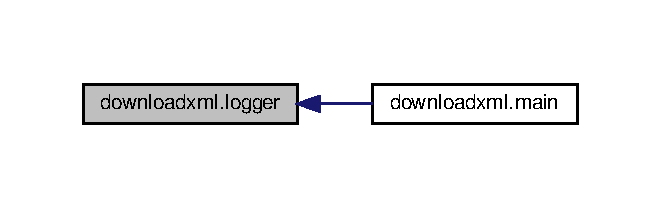
\includegraphics[width=317pt]{namespacedownloadxml_abc3f6c8d51f9a903bb8504a7ad9ad2de_icgraph}
\end{center}
\end{figure}
\mbox{\Hypertarget{namespacedownloadxml_ac0d6bf93a1be6263a0b94ef18bb9c459}\label{namespacedownloadxml_ac0d6bf93a1be6263a0b94ef18bb9c459}} 
\index{downloadxml@{downloadxml}!main@{main}}
\index{main@{main}!downloadxml@{downloadxml}}
\subsubsection{\texorpdfstring{main()}{main()}}
{\footnotesize\ttfamily def downloadxml.\+main (\begin{DoxyParamCaption}{ }\end{DoxyParamCaption})}



См. определение в файле downloadxml.\+py строка 103

Граф вызовов\+:\nopagebreak
\begin{figure}[H]
\begin{center}
\leavevmode
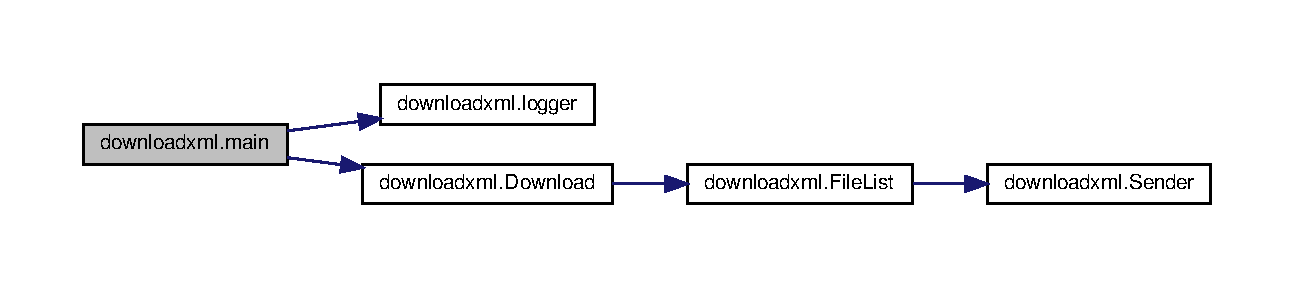
\includegraphics[width=350pt]{namespacedownloadxml_ac0d6bf93a1be6263a0b94ef18bb9c459_cgraph}
\end{center}
\end{figure}
\mbox{\Hypertarget{namespacedownloadxml_a7f19cfa93073885f474cf6a2a3f25e7f}\label{namespacedownloadxml_a7f19cfa93073885f474cf6a2a3f25e7f}} 
\index{downloadxml@{downloadxml}!Sender@{Sender}}
\index{Sender@{Sender}!downloadxml@{downloadxml}}
\subsubsection{\texorpdfstring{Sender()}{Sender()}}
{\footnotesize\ttfamily def downloadxml.\+Sender (\begin{DoxyParamCaption}\item[{}]{file }\end{DoxyParamCaption})}



Перемещение файлов и отправка в базу данных. 

Отправка полученного файла базу данных. Перемещение файлов из папки \textquotesingle{}../\+I\+N/\+C\+I\+C/\textquotesingle{} в \textquotesingle{}../\+O\+U\+T/\+C\+I\+C/\textquotesingle{} 

См. определение в файле downloadxml.\+py строка 60

Граф вызова функции\+:\nopagebreak
\begin{figure}[H]
\begin{center}
\leavevmode
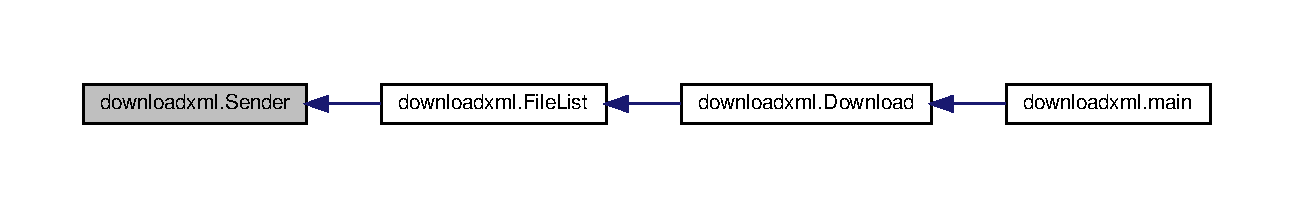
\includegraphics[width=350pt]{namespacedownloadxml_a7f19cfa93073885f474cf6a2a3f25e7f_icgraph}
\end{center}
\end{figure}


\subsection{Переменные}
\mbox{\Hypertarget{namespacedownloadxml_a75453296d7099653f232694ed5824b3f}\label{namespacedownloadxml_a75453296d7099653f232694ed5824b3f}} 
\index{downloadxml@{downloadxml}!dbhost@{dbhost}}
\index{dbhost@{dbhost}!downloadxml@{downloadxml}}
\subsubsection{\texorpdfstring{dbhost}{dbhost}}
{\footnotesize\ttfamily string downloadxml.\+dbhost = \textquotesingle{}localhost\textquotesingle{}}



См. определение в файле downloadxml.\+py строка 9

\mbox{\Hypertarget{namespacedownloadxml_ab0bd228b1313bba2e1fe1caa883e5b6c}\label{namespacedownloadxml_ab0bd228b1313bba2e1fe1caa883e5b6c}} 
\index{downloadxml@{downloadxml}!dbname@{dbname}}
\index{dbname@{dbname}!downloadxml@{downloadxml}}
\subsubsection{\texorpdfstring{dbname}{dbname}}
{\footnotesize\ttfamily string downloadxml.\+dbname = \textquotesingle{}project\+\_\+0\textquotesingle{}}



См. определение в файле downloadxml.\+py строка 13

\mbox{\Hypertarget{namespacedownloadxml_af527b05230cf500f27f1a899351d60af}\label{namespacedownloadxml_af527b05230cf500f27f1a899351d60af}} 
\index{downloadxml@{downloadxml}!dbpass@{dbpass}}
\index{dbpass@{dbpass}!downloadxml@{downloadxml}}
\subsubsection{\texorpdfstring{dbpass}{dbpass}}
{\footnotesize\ttfamily string downloadxml.\+dbpass = \textquotesingle{}1234\textquotesingle{}}



См. определение в файле downloadxml.\+py строка 12

\mbox{\Hypertarget{namespacedownloadxml_a32bdf9e8d022578666b5b9993714c4ef}\label{namespacedownloadxml_a32bdf9e8d022578666b5b9993714c4ef}} 
\index{downloadxml@{downloadxml}!dbport@{dbport}}
\index{dbport@{dbport}!downloadxml@{downloadxml}}
\subsubsection{\texorpdfstring{dbport}{dbport}}
{\footnotesize\ttfamily string downloadxml.\+dbport = \textquotesingle{}5432\textquotesingle{}}



См. определение в файле downloadxml.\+py строка 10

\mbox{\Hypertarget{namespacedownloadxml_ae0187d21bda573cccc7c253c38ac9494}\label{namespacedownloadxml_ae0187d21bda573cccc7c253c38ac9494}} 
\index{downloadxml@{downloadxml}!dbuser@{dbuser}}
\index{dbuser@{dbuser}!downloadxml@{downloadxml}}
\subsubsection{\texorpdfstring{dbuser}{dbuser}}
{\footnotesize\ttfamily string downloadxml.\+dbuser = \textquotesingle{}postgres\textquotesingle{}}



См. определение в файле downloadxml.\+py строка 11

\mbox{\Hypertarget{namespacedownloadxml_ae93409e2d65411e5e0c56c338629a095}\label{namespacedownloadxml_ae93409e2d65411e5e0c56c338629a095}} 
\index{downloadxml@{downloadxml}!Move\+Dir@{Move\+Dir}}
\index{Move\+Dir@{Move\+Dir}!downloadxml@{downloadxml}}
\subsubsection{\texorpdfstring{Move\+Dir}{MoveDir}}
{\footnotesize\ttfamily string downloadxml.\+Move\+Dir = \textquotesingle{}../O\+UT/C\+IC/\textquotesingle{}}



См. определение в файле downloadxml.\+py строка 16

\mbox{\Hypertarget{namespacedownloadxml_ac658e5e8b5ee862abc49621fce2f449a}\label{namespacedownloadxml_ac658e5e8b5ee862abc49621fce2f449a}} 
\index{downloadxml@{downloadxml}!Save\+Dir@{Save\+Dir}}
\index{Save\+Dir@{Save\+Dir}!downloadxml@{downloadxml}}
\subsubsection{\texorpdfstring{Save\+Dir}{SaveDir}}
{\footnotesize\ttfamily string downloadxml.\+Save\+Dir = \textquotesingle{}../IN/C\+IC/\textquotesingle{}}



См. определение в файле downloadxml.\+py строка 15

\mbox{\Hypertarget{namespacedownloadxml_a664dcd7a63115699604c60cc1c94b6db}\label{namespacedownloadxml_a664dcd7a63115699604c60cc1c94b6db}} 
\index{downloadxml@{downloadxml}!Sleep@{Sleep}}
\index{Sleep@{Sleep}!downloadxml@{downloadxml}}
\subsubsection{\texorpdfstring{Sleep}{Sleep}}
{\footnotesize\ttfamily int downloadxml.\+Sleep = 86400}



См. определение в файле downloadxml.\+py строка 20

\mbox{\Hypertarget{namespacedownloadxml_a89324d9cb91e8b04605a33cb8a959ac9}\label{namespacedownloadxml_a89324d9cb91e8b04605a33cb8a959ac9}} 
\index{downloadxml@{downloadxml}!urls@{urls}}
\index{urls@{urls}!downloadxml@{downloadxml}}
\subsubsection{\texorpdfstring{urls}{urls}}
{\footnotesize\ttfamily list downloadxml.\+urls = \mbox{[}\textquotesingle{}http\+://bdu.\+fstec.\+ru/documents/files/vulxml.\+zip\textquotesingle{}, \textquotesingle{}http\+://cve.\+mitre.\+org/data/downloads/allitems.\+xml.\+gz\textquotesingle{}\mbox{]}}



См. определение в файле downloadxml.\+py строка 19


\hypertarget{namespaceextractip}{}\section{Пространство имен extractip}
\label{namespaceextractip}\index{extractip@{extractip}}
\subsection*{Функции}
\begin{DoxyCompactItemize}
\item 
def \hyperlink{namespaceextractip_ad06d305b46e8793c42d3b69a019b024a}{logger} ()
\begin{DoxyCompactList}\small\item\em Запуск логгера. \end{DoxyCompactList}\item 
def \hyperlink{namespaceextractip_a027ec0c1479a189825c3ddcfefa0622d}{Int\+To\+IP} (ipnum)
\begin{DoxyCompactList}\small\item\em Преобразование из I\+N\+T\+E\+G\+ER в IP. \end{DoxyCompactList}\item 
def \hyperlink{namespaceextractip_a618ef8385421a257b0d4e90b39fd6050}{extract\+Ip} (fpath)
\begin{DoxyCompactList}\small\item\em Создание набора IP. \end{DoxyCompactList}\item 
def \hyperlink{namespaceextractip_a93e2b267d1b4fe1cef5c09f3b66217c0}{register} (f)
\begin{DoxyCompactList}\small\item\em Перенос файлов из I\+N/\+I\+PB в O\+U\+T/\+I\+PB. \end{DoxyCompactList}\item 
def \hyperlink{namespaceextractip_a4eeaa038e0dc125d55e221ea90a5a466}{send\+DB} ()
\begin{DoxyCompactList}\small\item\em Второй поток -\/ отправка в базу дананных. \end{DoxyCompactList}\item 
def \hyperlink{namespaceextractip_a3683febfdca5f525d87e4066e121b146}{prog} ()
\begin{DoxyCompactList}\small\item\em Первый поток -\/ обработка файлов. \end{DoxyCompactList}\item 
def \hyperlink{namespaceextractip_a4400b3ea86ebdf89264ad2424ca152e4}{main} ()
\begin{DoxyCompactList}\small\item\em Программа для чтения и преобразования файлов с IP и записи их в базу данных. \end{DoxyCompactList}\end{DoxyCompactItemize}
\subsection*{Переменные}
\begin{DoxyCompactItemize}
\item 
string \hyperlink{namespaceextractip_a3145a105043353658277d58cb99ff1c6}{indir} = \textquotesingle{}../IN/I\+PB\textquotesingle{}
\item 
string \hyperlink{namespaceextractip_afc77b990583eaef27725f54b1e371fd4}{f\+Dir} = \textquotesingle{}..//IN//I\+PB\textquotesingle{}
\item 
string \hyperlink{namespaceextractip_a990ac0d0fba3b9b0eff9e0538af6d7cf}{outdir} = \textquotesingle{}../O\+UT/I\+PB\textquotesingle{}
\item 
string \hyperlink{namespaceextractip_acbf601a19f64d09908d5ab149094b94d}{r\+Back} = \textquotesingle{}../IN/\textquotesingle{}
\item 
string \hyperlink{namespaceextractip_ac577365c0a3822c9a30c2f72ecd62c18}{dbhost} = \textquotesingle{}localhost\textquotesingle{}
\item 
string \hyperlink{namespaceextractip_a37c1fd9eb8523d6a57cbd077d2075be2}{dbport} = \textquotesingle{}5432\textquotesingle{}
\item 
string \hyperlink{namespaceextractip_ae958c259d1ade44ffc42dc20f7d4b3ab}{dbuser} = \textquotesingle{}postgres\textquotesingle{}
\item 
string \hyperlink{namespaceextractip_a1cc5f8cfee8451384713192bae5cf558}{dbpass} = \textquotesingle{}postgres\textquotesingle{}
\item 
string \hyperlink{namespaceextractip_a9394808f1a48ea90bfa2bb86c76d01ad}{dbname} = \textquotesingle{}project\+\_\+0\textquotesingle{}
\item 
\hyperlink{namespaceextractip_a2cf221bd199a42f6c0e3a42cba40b841}{q} = queue.\+Queue()
\end{DoxyCompactItemize}


\subsection{Функции}
\mbox{\Hypertarget{namespaceextractip_a618ef8385421a257b0d4e90b39fd6050}\label{namespaceextractip_a618ef8385421a257b0d4e90b39fd6050}} 
\index{extractip@{extractip}!extract\+Ip@{extract\+Ip}}
\index{extract\+Ip@{extract\+Ip}!extractip@{extractip}}
\subsubsection{\texorpdfstring{extract\+Ip()}{extractIp()}}
{\footnotesize\ttfamily def extractip.\+extract\+Ip (\begin{DoxyParamCaption}\item[{}]{fpath }\end{DoxyParamCaption})}



Создание набора IP. 



См. определение в файле extractip.\+py строка 49

Граф вызовов\+:\nopagebreak
\begin{figure}[H]
\begin{center}
\leavevmode
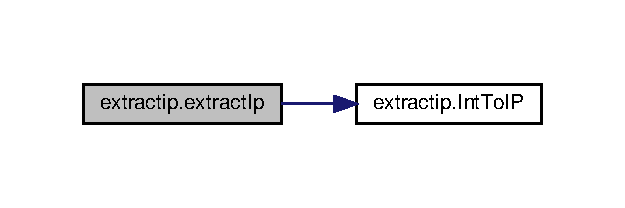
\includegraphics[width=300pt]{namespaceextractip_a618ef8385421a257b0d4e90b39fd6050_cgraph}
\end{center}
\end{figure}
Граф вызова функции\+:\nopagebreak
\begin{figure}[H]
\begin{center}
\leavevmode
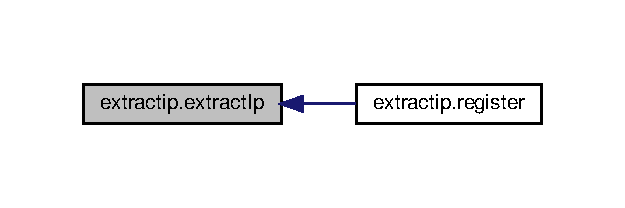
\includegraphics[width=300pt]{namespaceextractip_a618ef8385421a257b0d4e90b39fd6050_icgraph}
\end{center}
\end{figure}
\mbox{\Hypertarget{namespaceextractip_a027ec0c1479a189825c3ddcfefa0622d}\label{namespaceextractip_a027ec0c1479a189825c3ddcfefa0622d}} 
\index{extractip@{extractip}!Int\+To\+IP@{Int\+To\+IP}}
\index{Int\+To\+IP@{Int\+To\+IP}!extractip@{extractip}}
\subsubsection{\texorpdfstring{Int\+To\+I\+P()}{IntToIP()}}
{\footnotesize\ttfamily def extractip.\+Int\+To\+IP (\begin{DoxyParamCaption}\item[{}]{ipnum }\end{DoxyParamCaption})}



Преобразование из I\+N\+T\+E\+G\+ER в IP. 



См. определение в файле extractip.\+py строка 38

Граф вызова функции\+:\nopagebreak
\begin{figure}[H]
\begin{center}
\leavevmode
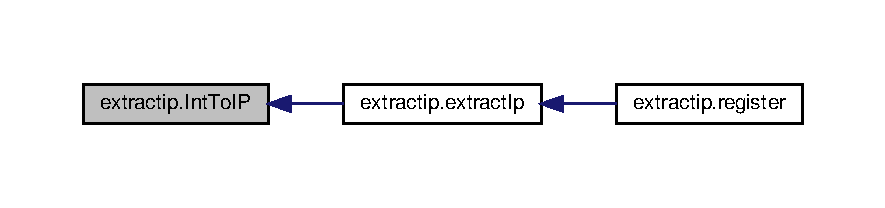
\includegraphics[width=350pt]{namespaceextractip_a027ec0c1479a189825c3ddcfefa0622d_icgraph}
\end{center}
\end{figure}
\mbox{\Hypertarget{namespaceextractip_ad06d305b46e8793c42d3b69a019b024a}\label{namespaceextractip_ad06d305b46e8793c42d3b69a019b024a}} 
\index{extractip@{extractip}!logger@{logger}}
\index{logger@{logger}!extractip@{extractip}}
\subsubsection{\texorpdfstring{logger()}{logger()}}
{\footnotesize\ttfamily def extractip.\+logger (\begin{DoxyParamCaption}{ }\end{DoxyParamCaption})}



Запуск логгера. 



См. определение в файле extractip.\+py строка 29

Граф вызова функции\+:\nopagebreak
\begin{figure}[H]
\begin{center}
\leavevmode
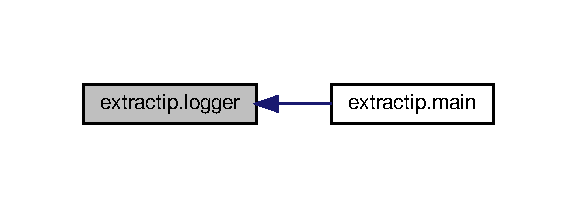
\includegraphics[width=277pt]{namespaceextractip_ad06d305b46e8793c42d3b69a019b024a_icgraph}
\end{center}
\end{figure}
\mbox{\Hypertarget{namespaceextractip_a4400b3ea86ebdf89264ad2424ca152e4}\label{namespaceextractip_a4400b3ea86ebdf89264ad2424ca152e4}} 
\index{extractip@{extractip}!main@{main}}
\index{main@{main}!extractip@{extractip}}
\subsubsection{\texorpdfstring{main()}{main()}}
{\footnotesize\ttfamily def extractip.\+main (\begin{DoxyParamCaption}{ }\end{DoxyParamCaption})}



Программа для чтения и преобразования файлов с IP и записи их в базу данных. 

При запуске запускается логгер и 2 основных потока. 

См. определение в файле extractip.\+py строка 146

Граф вызовов\+:\nopagebreak
\begin{figure}[H]
\begin{center}
\leavevmode
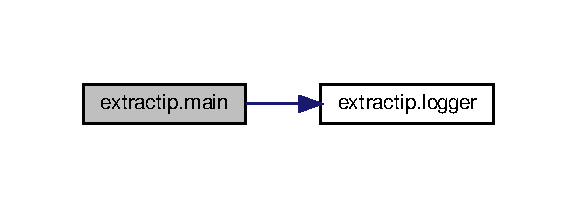
\includegraphics[width=277pt]{namespaceextractip_a4400b3ea86ebdf89264ad2424ca152e4_cgraph}
\end{center}
\end{figure}
\mbox{\Hypertarget{namespaceextractip_a3683febfdca5f525d87e4066e121b146}\label{namespaceextractip_a3683febfdca5f525d87e4066e121b146}} 
\index{extractip@{extractip}!prog@{prog}}
\index{prog@{prog}!extractip@{extractip}}
\subsubsection{\texorpdfstring{prog()}{prog()}}
{\footnotesize\ttfamily def extractip.\+prog (\begin{DoxyParamCaption}{ }\end{DoxyParamCaption})}



Первый поток -\/ обработка файлов. 

Ищет входящие файлы и запускает еще шесть потоков для первых 1000 файлов. Добавляет результаты в очередь и исключает повторные I\+Ps. Обработка следующих 1000 файлов. Если нет входящих файлов, то ждем появления элементов. 

См. определение в файле extractip.\+py строка 121

\mbox{\Hypertarget{namespaceextractip_a93e2b267d1b4fe1cef5c09f3b66217c0}\label{namespaceextractip_a93e2b267d1b4fe1cef5c09f3b66217c0}} 
\index{extractip@{extractip}!register@{register}}
\index{register@{register}!extractip@{extractip}}
\subsubsection{\texorpdfstring{register()}{register()}}
{\footnotesize\ttfamily def extractip.\+register (\begin{DoxyParamCaption}\item[{}]{f }\end{DoxyParamCaption})}



Перенос файлов из I\+N/\+I\+PB в O\+U\+T/\+I\+PB. 

Файлы которые невозможно прочесть выбрасываются в родительскую папку IN. 

См. определение в файле extractip.\+py строка 67

Граф вызовов\+:\nopagebreak
\begin{figure}[H]
\begin{center}
\leavevmode
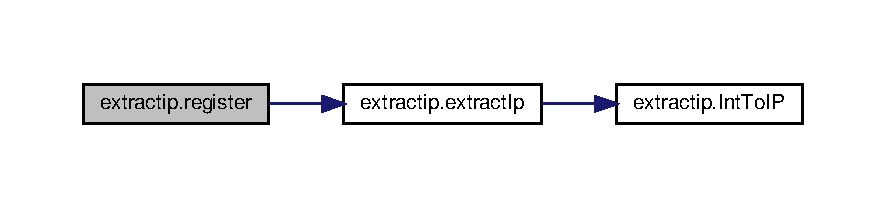
\includegraphics[width=350pt]{namespaceextractip_a93e2b267d1b4fe1cef5c09f3b66217c0_cgraph}
\end{center}
\end{figure}
\mbox{\Hypertarget{namespaceextractip_a4eeaa038e0dc125d55e221ea90a5a466}\label{namespaceextractip_a4eeaa038e0dc125d55e221ea90a5a466}} 
\index{extractip@{extractip}!send\+DB@{send\+DB}}
\index{send\+DB@{send\+DB}!extractip@{extractip}}
\subsubsection{\texorpdfstring{send\+D\+B()}{sendDB()}}
{\footnotesize\ttfamily def extractip.\+send\+DB (\begin{DoxyParamCaption}{ }\end{DoxyParamCaption})}



Второй поток -\/ отправка в базу дананных. 

Получение элементов из очереди. Создание соединения с базой данных. Отправка полученного набора IP в базу данных. Ожидание следующего списка элементов. 

См. определение в файле extractip.\+py строка 85



\subsection{Переменные}
\mbox{\Hypertarget{namespaceextractip_ac577365c0a3822c9a30c2f72ecd62c18}\label{namespaceextractip_ac577365c0a3822c9a30c2f72ecd62c18}} 
\index{extractip@{extractip}!dbhost@{dbhost}}
\index{dbhost@{dbhost}!extractip@{extractip}}
\subsubsection{\texorpdfstring{dbhost}{dbhost}}
{\footnotesize\ttfamily string extractip.\+dbhost = \textquotesingle{}localhost\textquotesingle{}}



См. определение в файле extractip.\+py строка 17

\mbox{\Hypertarget{namespaceextractip_a9394808f1a48ea90bfa2bb86c76d01ad}\label{namespaceextractip_a9394808f1a48ea90bfa2bb86c76d01ad}} 
\index{extractip@{extractip}!dbname@{dbname}}
\index{dbname@{dbname}!extractip@{extractip}}
\subsubsection{\texorpdfstring{dbname}{dbname}}
{\footnotesize\ttfamily string extractip.\+dbname = \textquotesingle{}project\+\_\+0\textquotesingle{}}



См. определение в файле extractip.\+py строка 21

\mbox{\Hypertarget{namespaceextractip_a1cc5f8cfee8451384713192bae5cf558}\label{namespaceextractip_a1cc5f8cfee8451384713192bae5cf558}} 
\index{extractip@{extractip}!dbpass@{dbpass}}
\index{dbpass@{dbpass}!extractip@{extractip}}
\subsubsection{\texorpdfstring{dbpass}{dbpass}}
{\footnotesize\ttfamily string extractip.\+dbpass = \textquotesingle{}postgres\textquotesingle{}}



См. определение в файле extractip.\+py строка 20

\mbox{\Hypertarget{namespaceextractip_a37c1fd9eb8523d6a57cbd077d2075be2}\label{namespaceextractip_a37c1fd9eb8523d6a57cbd077d2075be2}} 
\index{extractip@{extractip}!dbport@{dbport}}
\index{dbport@{dbport}!extractip@{extractip}}
\subsubsection{\texorpdfstring{dbport}{dbport}}
{\footnotesize\ttfamily string extractip.\+dbport = \textquotesingle{}5432\textquotesingle{}}



См. определение в файле extractip.\+py строка 18

\mbox{\Hypertarget{namespaceextractip_ae958c259d1ade44ffc42dc20f7d4b3ab}\label{namespaceextractip_ae958c259d1ade44ffc42dc20f7d4b3ab}} 
\index{extractip@{extractip}!dbuser@{dbuser}}
\index{dbuser@{dbuser}!extractip@{extractip}}
\subsubsection{\texorpdfstring{dbuser}{dbuser}}
{\footnotesize\ttfamily string extractip.\+dbuser = \textquotesingle{}postgres\textquotesingle{}}



См. определение в файле extractip.\+py строка 19

\mbox{\Hypertarget{namespaceextractip_afc77b990583eaef27725f54b1e371fd4}\label{namespaceextractip_afc77b990583eaef27725f54b1e371fd4}} 
\index{extractip@{extractip}!f\+Dir@{f\+Dir}}
\index{f\+Dir@{f\+Dir}!extractip@{extractip}}
\subsubsection{\texorpdfstring{f\+Dir}{fDir}}
{\footnotesize\ttfamily string extractip.\+f\+Dir = \textquotesingle{}..//IN//I\+PB\textquotesingle{}}



См. определение в файле extractip.\+py строка 14

\mbox{\Hypertarget{namespaceextractip_a3145a105043353658277d58cb99ff1c6}\label{namespaceextractip_a3145a105043353658277d58cb99ff1c6}} 
\index{extractip@{extractip}!indir@{indir}}
\index{indir@{indir}!extractip@{extractip}}
\subsubsection{\texorpdfstring{indir}{indir}}
{\footnotesize\ttfamily string extractip.\+indir = \textquotesingle{}../IN/I\+PB\textquotesingle{}}



См. определение в файле extractip.\+py строка 13

\mbox{\Hypertarget{namespaceextractip_a990ac0d0fba3b9b0eff9e0538af6d7cf}\label{namespaceextractip_a990ac0d0fba3b9b0eff9e0538af6d7cf}} 
\index{extractip@{extractip}!outdir@{outdir}}
\index{outdir@{outdir}!extractip@{extractip}}
\subsubsection{\texorpdfstring{outdir}{outdir}}
{\footnotesize\ttfamily string extractip.\+outdir = \textquotesingle{}../O\+UT/I\+PB\textquotesingle{}}



См. определение в файле extractip.\+py строка 15

\mbox{\Hypertarget{namespaceextractip_a2cf221bd199a42f6c0e3a42cba40b841}\label{namespaceextractip_a2cf221bd199a42f6c0e3a42cba40b841}} 
\index{extractip@{extractip}!q@{q}}
\index{q@{q}!extractip@{extractip}}
\subsubsection{\texorpdfstring{q}{q}}
{\footnotesize\ttfamily extractip.\+q = queue.\+Queue()}



См. определение в файле extractip.\+py строка 23

\mbox{\Hypertarget{namespaceextractip_acbf601a19f64d09908d5ab149094b94d}\label{namespaceextractip_acbf601a19f64d09908d5ab149094b94d}} 
\index{extractip@{extractip}!r\+Back@{r\+Back}}
\index{r\+Back@{r\+Back}!extractip@{extractip}}
\subsubsection{\texorpdfstring{r\+Back}{rBack}}
{\footnotesize\ttfamily string extractip.\+r\+Back = \textquotesingle{}../IN/\textquotesingle{}}



См. определение в файле extractip.\+py строка 16


\hypertarget{namespacerecognizeip}{}\section{Пространство имен recognizeip}
\label{namespacerecognizeip}\index{recognizeip@{recognizeip}}
\subsection*{Функции}
\begin{DoxyCompactItemize}
\item 
def \hyperlink{namespacerecognizeip_a99d8f7a73addea7cea8ad5b0225e5005}{logger} ()
\begin{DoxyCompactList}\small\item\em Запуск логгера. \end{DoxyCompactList}\item 
def \hyperlink{namespacerecognizeip_a3bb8e2d63860a9c4027908b34014c56b}{Get\+Unknown} ()
\begin{DoxyCompactList}\small\item\em Получение неизвестных IP из базы данных. \end{DoxyCompactList}\item 
def \hyperlink{namespacerecognizeip_a362c41c14e0d237c722ab6c2234d6afa}{Get\+Request} (res)
\begin{DoxyCompactList}\small\item\em Отправка IP на сервер и получение json\textquotesingle{}a с информацией об этих IP. \end{DoxyCompactList}\item 
def \hyperlink{namespacerecognizeip_a7055bdccbd846aa71a7be77513548e08}{Update\+Unknown} (ip, cntry, cde, city, lat, lon)
\begin{DoxyCompactList}\small\item\em Обновление IP в базе данных. \end{DoxyCompactList}\item 
def \hyperlink{namespacerecognizeip_ad9b913f5fd7d2c429fb56302952d3d74}{Parse\+Json} (ips)
\begin{DoxyCompactList}\small\item\em Чтение json\textquotesingle{}a. \end{DoxyCompactList}\item 
def \hyperlink{namespacerecognizeip_a9fb9f625acd36513818c1ac2f236070d}{scan} ()
\begin{DoxyCompactList}\small\item\em Ожидание неизвестх IP. \end{DoxyCompactList}\item 
def \hyperlink{namespacerecognizeip_af2c16760c67e840d48d82917a9c9cacb}{updatedate} ()
\begin{DoxyCompactList}\small\item\em Обновление даты IP в базе данных. \end{DoxyCompactList}\item 
def \hyperlink{namespacerecognizeip_aeacb92c088c1e5c9894254e390bc52c2}{main} ()
\begin{DoxyCompactList}\small\item\em Программа для получения информации о неизвестных I\+P-\/адресов. \end{DoxyCompactList}\end{DoxyCompactItemize}
\subsection*{Переменные}
\begin{DoxyCompactItemize}
\item 
string \hyperlink{namespacerecognizeip_ab088007f4af084f71c33ab23b8aa59fe}{dbhost} = \textquotesingle{}localhost\textquotesingle{}
\item 
string \hyperlink{namespacerecognizeip_ae2d5ad4fcc3fcd7393e4a18f53282798}{dbport} = \textquotesingle{}5432\textquotesingle{}
\item 
string \hyperlink{namespacerecognizeip_acc52b089af5fa13c73a78f70daa56494}{dbuser} = \textquotesingle{}postgres\textquotesingle{}
\item 
string \hyperlink{namespacerecognizeip_a4ed50ea7f07921938765ea73e8131467}{dbpass} = \textquotesingle{}postgres\textquotesingle{}
\item 
string \hyperlink{namespacerecognizeip_a114539cfda8487773400a49df2653b25}{dbname} = \textquotesingle{}project\+\_\+0\textquotesingle{}
\item 
int \hyperlink{namespacerecognizeip_ad79dcdb5a4cb450c8945c8fe3185e85a}{Sleep} = 86400
\end{DoxyCompactItemize}


\subsection{Функции}
\mbox{\Hypertarget{namespacerecognizeip_a362c41c14e0d237c722ab6c2234d6afa}\label{namespacerecognizeip_a362c41c14e0d237c722ab6c2234d6afa}} 
\index{recognizeip@{recognizeip}!Get\+Request@{Get\+Request}}
\index{Get\+Request@{Get\+Request}!recognizeip@{recognizeip}}
\subsubsection{\texorpdfstring{Get\+Request()}{GetRequest()}}
{\footnotesize\ttfamily def recognizeip.\+Get\+Request (\begin{DoxyParamCaption}\item[{}]{res }\end{DoxyParamCaption})}



Отправка IP на сервер и получение json\textquotesingle{}a с информацией об этих IP. 



См. определение в файле recognizeip.\+py строка 55

Граф вызова функции\+:\nopagebreak
\begin{figure}[H]
\begin{center}
\leavevmode
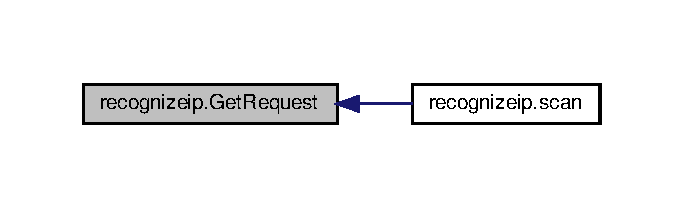
\includegraphics[width=328pt]{namespacerecognizeip_a362c41c14e0d237c722ab6c2234d6afa_icgraph}
\end{center}
\end{figure}
\mbox{\Hypertarget{namespacerecognizeip_a3bb8e2d63860a9c4027908b34014c56b}\label{namespacerecognizeip_a3bb8e2d63860a9c4027908b34014c56b}} 
\index{recognizeip@{recognizeip}!Get\+Unknown@{Get\+Unknown}}
\index{Get\+Unknown@{Get\+Unknown}!recognizeip@{recognizeip}}
\subsubsection{\texorpdfstring{Get\+Unknown()}{GetUnknown()}}
{\footnotesize\ttfamily def recognizeip.\+Get\+Unknown (\begin{DoxyParamCaption}{ }\end{DoxyParamCaption})}



Получение неизвестных IP из базы данных. 



См. определение в файле recognizeip.\+py строка 31

Граф вызова функции\+:\nopagebreak
\begin{figure}[H]
\begin{center}
\leavevmode
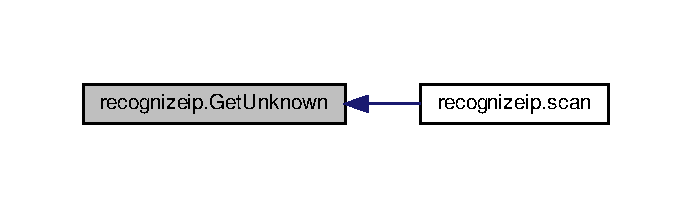
\includegraphics[width=332pt]{namespacerecognizeip_a3bb8e2d63860a9c4027908b34014c56b_icgraph}
\end{center}
\end{figure}
\mbox{\Hypertarget{namespacerecognizeip_a99d8f7a73addea7cea8ad5b0225e5005}\label{namespacerecognizeip_a99d8f7a73addea7cea8ad5b0225e5005}} 
\index{recognizeip@{recognizeip}!logger@{logger}}
\index{logger@{logger}!recognizeip@{recognizeip}}
\subsubsection{\texorpdfstring{logger()}{logger()}}
{\footnotesize\ttfamily def recognizeip.\+logger (\begin{DoxyParamCaption}{ }\end{DoxyParamCaption})}



Запуск логгера. 



См. определение в файле recognizeip.\+py строка 19

Граф вызова функции\+:\nopagebreak
\begin{figure}[H]
\begin{center}
\leavevmode
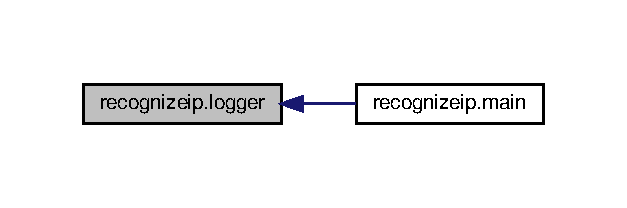
\includegraphics[width=301pt]{namespacerecognizeip_a99d8f7a73addea7cea8ad5b0225e5005_icgraph}
\end{center}
\end{figure}
\mbox{\Hypertarget{namespacerecognizeip_aeacb92c088c1e5c9894254e390bc52c2}\label{namespacerecognizeip_aeacb92c088c1e5c9894254e390bc52c2}} 
\index{recognizeip@{recognizeip}!main@{main}}
\index{main@{main}!recognizeip@{recognizeip}}
\subsubsection{\texorpdfstring{main()}{main()}}
{\footnotesize\ttfamily def recognizeip.\+main (\begin{DoxyParamCaption}{ }\end{DoxyParamCaption})}



Программа для получения информации о неизвестных I\+P-\/адресов. 



См. определение в файле recognizeip.\+py строка 155

Граф вызовов\+:\nopagebreak
\begin{figure}[H]
\begin{center}
\leavevmode
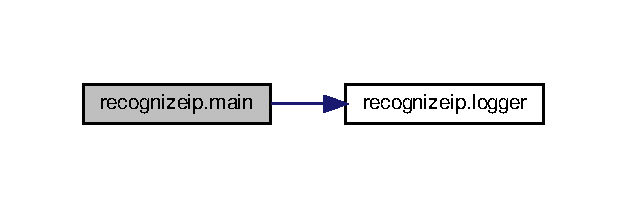
\includegraphics[width=301pt]{namespacerecognizeip_aeacb92c088c1e5c9894254e390bc52c2_cgraph}
\end{center}
\end{figure}
\mbox{\Hypertarget{namespacerecognizeip_ad9b913f5fd7d2c429fb56302952d3d74}\label{namespacerecognizeip_ad9b913f5fd7d2c429fb56302952d3d74}} 
\index{recognizeip@{recognizeip}!Parse\+Json@{Parse\+Json}}
\index{Parse\+Json@{Parse\+Json}!recognizeip@{recognizeip}}
\subsubsection{\texorpdfstring{Parse\+Json()}{ParseJson()}}
{\footnotesize\ttfamily def recognizeip.\+Parse\+Json (\begin{DoxyParamCaption}\item[{}]{ips }\end{DoxyParamCaption})}



Чтение json\textquotesingle{}a. 



См. определение в файле recognizeip.\+py строка 94

Граф вызовов\+:\nopagebreak
\begin{figure}[H]
\begin{center}
\leavevmode
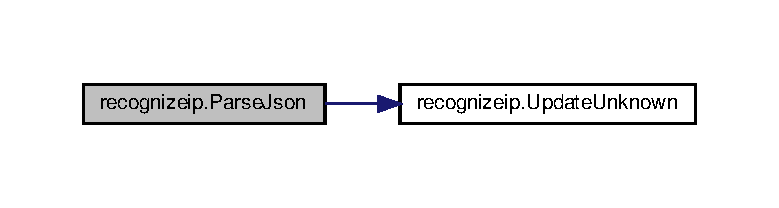
\includegraphics[width=350pt]{namespacerecognizeip_ad9b913f5fd7d2c429fb56302952d3d74_cgraph}
\end{center}
\end{figure}
Граф вызова функции\+:\nopagebreak
\begin{figure}[H]
\begin{center}
\leavevmode
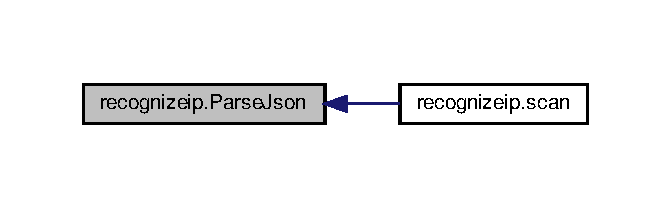
\includegraphics[width=322pt]{namespacerecognizeip_ad9b913f5fd7d2c429fb56302952d3d74_icgraph}
\end{center}
\end{figure}
\mbox{\Hypertarget{namespacerecognizeip_a9fb9f625acd36513818c1ac2f236070d}\label{namespacerecognizeip_a9fb9f625acd36513818c1ac2f236070d}} 
\index{recognizeip@{recognizeip}!scan@{scan}}
\index{scan@{scan}!recognizeip@{recognizeip}}
\subsubsection{\texorpdfstring{scan()}{scan()}}
{\footnotesize\ttfamily def recognizeip.\+scan (\begin{DoxyParamCaption}{ }\end{DoxyParamCaption})}



Ожидание неизвестх IP. 



См. определение в файле recognizeip.\+py строка 121

Граф вызовов\+:\nopagebreak
\begin{figure}[H]
\begin{center}
\leavevmode
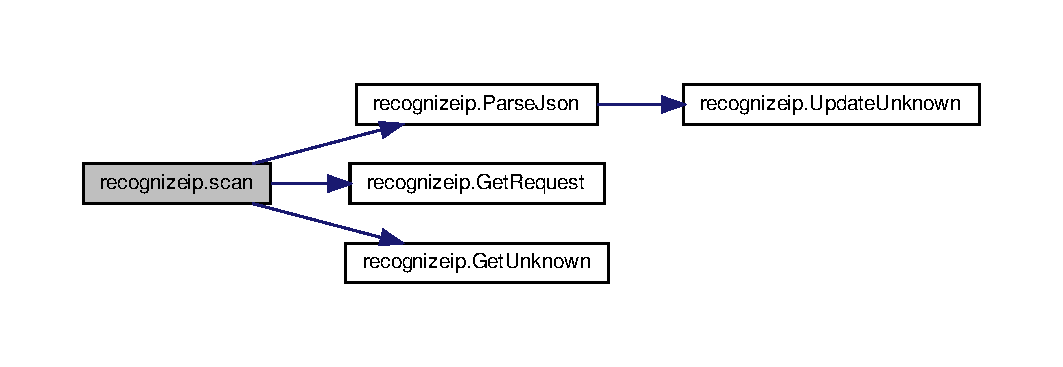
\includegraphics[width=350pt]{namespacerecognizeip_a9fb9f625acd36513818c1ac2f236070d_cgraph}
\end{center}
\end{figure}
\mbox{\Hypertarget{namespacerecognizeip_af2c16760c67e840d48d82917a9c9cacb}\label{namespacerecognizeip_af2c16760c67e840d48d82917a9c9cacb}} 
\index{recognizeip@{recognizeip}!updatedate@{updatedate}}
\index{updatedate@{updatedate}!recognizeip@{recognizeip}}
\subsubsection{\texorpdfstring{updatedate()}{updatedate()}}
{\footnotesize\ttfamily def recognizeip.\+updatedate (\begin{DoxyParamCaption}{ }\end{DoxyParamCaption})}



Обновление даты IP в базе данных. 



См. определение в файле recognizeip.\+py строка 131

\mbox{\Hypertarget{namespacerecognizeip_a7055bdccbd846aa71a7be77513548e08}\label{namespacerecognizeip_a7055bdccbd846aa71a7be77513548e08}} 
\index{recognizeip@{recognizeip}!Update\+Unknown@{Update\+Unknown}}
\index{Update\+Unknown@{Update\+Unknown}!recognizeip@{recognizeip}}
\subsubsection{\texorpdfstring{Update\+Unknown()}{UpdateUnknown()}}
{\footnotesize\ttfamily def recognizeip.\+Update\+Unknown (\begin{DoxyParamCaption}\item[{}]{ip,  }\item[{}]{cntry,  }\item[{}]{cde,  }\item[{}]{city,  }\item[{}]{lat,  }\item[{}]{lon }\end{DoxyParamCaption})}



Обновление IP в базе данных. 



См. определение в файле recognizeip.\+py строка 76

Граф вызова функции\+:\nopagebreak
\begin{figure}[H]
\begin{center}
\leavevmode
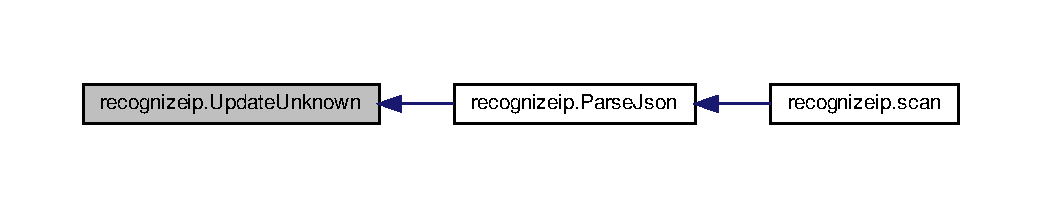
\includegraphics[width=350pt]{namespacerecognizeip_a7055bdccbd846aa71a7be77513548e08_icgraph}
\end{center}
\end{figure}


\subsection{Переменные}
\mbox{\Hypertarget{namespacerecognizeip_ab088007f4af084f71c33ab23b8aa59fe}\label{namespacerecognizeip_ab088007f4af084f71c33ab23b8aa59fe}} 
\index{recognizeip@{recognizeip}!dbhost@{dbhost}}
\index{dbhost@{dbhost}!recognizeip@{recognizeip}}
\subsubsection{\texorpdfstring{dbhost}{dbhost}}
{\footnotesize\ttfamily string recognizeip.\+dbhost = \textquotesingle{}localhost\textquotesingle{}}



См. определение в файле recognizeip.\+py строка 7

\mbox{\Hypertarget{namespacerecognizeip_a114539cfda8487773400a49df2653b25}\label{namespacerecognizeip_a114539cfda8487773400a49df2653b25}} 
\index{recognizeip@{recognizeip}!dbname@{dbname}}
\index{dbname@{dbname}!recognizeip@{recognizeip}}
\subsubsection{\texorpdfstring{dbname}{dbname}}
{\footnotesize\ttfamily string recognizeip.\+dbname = \textquotesingle{}project\+\_\+0\textquotesingle{}}



См. определение в файле recognizeip.\+py строка 11

\mbox{\Hypertarget{namespacerecognizeip_a4ed50ea7f07921938765ea73e8131467}\label{namespacerecognizeip_a4ed50ea7f07921938765ea73e8131467}} 
\index{recognizeip@{recognizeip}!dbpass@{dbpass}}
\index{dbpass@{dbpass}!recognizeip@{recognizeip}}
\subsubsection{\texorpdfstring{dbpass}{dbpass}}
{\footnotesize\ttfamily string recognizeip.\+dbpass = \textquotesingle{}postgres\textquotesingle{}}



См. определение в файле recognizeip.\+py строка 10

\mbox{\Hypertarget{namespacerecognizeip_ae2d5ad4fcc3fcd7393e4a18f53282798}\label{namespacerecognizeip_ae2d5ad4fcc3fcd7393e4a18f53282798}} 
\index{recognizeip@{recognizeip}!dbport@{dbport}}
\index{dbport@{dbport}!recognizeip@{recognizeip}}
\subsubsection{\texorpdfstring{dbport}{dbport}}
{\footnotesize\ttfamily string recognizeip.\+dbport = \textquotesingle{}5432\textquotesingle{}}



См. определение в файле recognizeip.\+py строка 8

\mbox{\Hypertarget{namespacerecognizeip_acc52b089af5fa13c73a78f70daa56494}\label{namespacerecognizeip_acc52b089af5fa13c73a78f70daa56494}} 
\index{recognizeip@{recognizeip}!dbuser@{dbuser}}
\index{dbuser@{dbuser}!recognizeip@{recognizeip}}
\subsubsection{\texorpdfstring{dbuser}{dbuser}}
{\footnotesize\ttfamily string recognizeip.\+dbuser = \textquotesingle{}postgres\textquotesingle{}}



См. определение в файле recognizeip.\+py строка 9

\mbox{\Hypertarget{namespacerecognizeip_ad79dcdb5a4cb450c8945c8fe3185e85a}\label{namespacerecognizeip_ad79dcdb5a4cb450c8945c8fe3185e85a}} 
\index{recognizeip@{recognizeip}!Sleep@{Sleep}}
\index{Sleep@{Sleep}!recognizeip@{recognizeip}}
\subsubsection{\texorpdfstring{Sleep}{Sleep}}
{\footnotesize\ttfamily int recognizeip.\+Sleep = 86400}



См. определение в файле recognizeip.\+py строка 13


\chapter{Файлы}
\hypertarget{availableurl_8py}{}\section{Файл availableurl.\+py}
\label{availableurl_8py}\index{availableurl.\+py@{availableurl.\+py}}
\subsection*{Пространства имен}
\begin{DoxyCompactItemize}
\item 
 \hyperlink{namespaceavailableurl}{availableurl}
\end{DoxyCompactItemize}
\subsection*{Функции}
\begin{DoxyCompactItemize}
\item 
def \hyperlink{namespaceavailableurl_a25d6c72ce2cd54a5490720f1319c68dc}{availableurl.\+logger} ()
\begin{DoxyCompactList}\small\item\em Запуск логгера. \end{DoxyCompactList}\item 
def \hyperlink{namespaceavailableurl_aff3d4545f3483782a407aab7859602f4}{availableurl.\+Access} ()
\begin{DoxyCompactList}\small\item\em Проверка доступности U\+R\+L-\/адресов. \end{DoxyCompactList}\item 
def \hyperlink{namespaceavailableurl_a9bdd46562a5ef06276fceee5109958e7}{availableurl.\+main} ()
\end{DoxyCompactItemize}
\subsection*{Переменные}
\begin{DoxyCompactItemize}
\item 
string \hyperlink{namespaceavailableurl_a37fb41a94b1d571e29110ace71a6779b}{availableurl.\+dbhost} = \textquotesingle{}localhost\textquotesingle{}
\item 
string \hyperlink{namespaceavailableurl_a390f7a9e2e87f1ef981f38c17606925a}{availableurl.\+dbport} = \textquotesingle{}5432\textquotesingle{}
\item 
string \hyperlink{namespaceavailableurl_a7aad22fecf6c516bded3d3c0a571bd40}{availableurl.\+dbuser} = \textquotesingle{}postgres\textquotesingle{}
\item 
string \hyperlink{namespaceavailableurl_a213229dedd788b05a4d417a6e54d5662}{availableurl.\+dbpass} = \textquotesingle{}1234\textquotesingle{}
\item 
string \hyperlink{namespaceavailableurl_ac13da61208e787ad038413b3779bf437}{availableurl.\+dbname} = \textquotesingle{}project\+\_\+0\textquotesingle{}
\end{DoxyCompactItemize}

\hypertarget{config_8dox}{}\section{Файл config.\+dox}
\label{config_8dox}\index{config.\+dox@{config.\+dox}}

\hypertarget{downloadxml_8py}{}\section{Файл downloadxml.\+py}
\label{downloadxml_8py}\index{downloadxml.\+py@{downloadxml.\+py}}
\subsection*{Пространства имен}
\begin{DoxyCompactItemize}
\item 
 \hyperlink{namespacedownloadxml}{downloadxml}
\end{DoxyCompactItemize}
\subsection*{Функции}
\begin{DoxyCompactItemize}
\item 
def \hyperlink{namespacedownloadxml_abc3f6c8d51f9a903bb8504a7ad9ad2de}{downloadxml.\+logger} ()
\begin{DoxyCompactList}\small\item\em Запуск логгера. \end{DoxyCompactList}\item 
def \hyperlink{namespacedownloadxml_a7f19cfa93073885f474cf6a2a3f25e7f}{downloadxml.\+Sender} (file)
\begin{DoxyCompactList}\small\item\em Перемещение файлов и отправка в базу данных. \end{DoxyCompactList}\item 
def \hyperlink{namespacedownloadxml_ae15b4d4f7f282d34e48e03a2452741d6}{downloadxml.\+File\+List} ()
\begin{DoxyCompactList}\small\item\em Получение списка xml-\/файлов. \end{DoxyCompactList}\item 
def \hyperlink{namespacedownloadxml_a801fc32a7254a9319cb06fb65fb757e9}{downloadxml.\+Download} ()
\begin{DoxyCompactList}\small\item\em Скачивание списоков угроз. \end{DoxyCompactList}\item 
def \hyperlink{namespacedownloadxml_ac0d6bf93a1be6263a0b94ef18bb9c459}{downloadxml.\+main} ()
\end{DoxyCompactItemize}
\subsection*{Переменные}
\begin{DoxyCompactItemize}
\item 
string \hyperlink{namespacedownloadxml_a75453296d7099653f232694ed5824b3f}{downloadxml.\+dbhost} = \textquotesingle{}localhost\textquotesingle{}
\item 
string \hyperlink{namespacedownloadxml_a32bdf9e8d022578666b5b9993714c4ef}{downloadxml.\+dbport} = \textquotesingle{}5432\textquotesingle{}
\item 
string \hyperlink{namespacedownloadxml_ae0187d21bda573cccc7c253c38ac9494}{downloadxml.\+dbuser} = \textquotesingle{}postgres\textquotesingle{}
\item 
string \hyperlink{namespacedownloadxml_af527b05230cf500f27f1a899351d60af}{downloadxml.\+dbpass} = \textquotesingle{}1234\textquotesingle{}
\item 
string \hyperlink{namespacedownloadxml_ab0bd228b1313bba2e1fe1caa883e5b6c}{downloadxml.\+dbname} = \textquotesingle{}project\+\_\+0\textquotesingle{}
\item 
string \hyperlink{namespacedownloadxml_ac658e5e8b5ee862abc49621fce2f449a}{downloadxml.\+Save\+Dir} = \textquotesingle{}../IN/C\+IC/\textquotesingle{}
\item 
string \hyperlink{namespacedownloadxml_ae93409e2d65411e5e0c56c338629a095}{downloadxml.\+Move\+Dir} = \textquotesingle{}../O\+UT/C\+IC/\textquotesingle{}
\item 
list \hyperlink{namespacedownloadxml_a89324d9cb91e8b04605a33cb8a959ac9}{downloadxml.\+urls} = \mbox{[}\textquotesingle{}http\+://bdu.\+fstec.\+ru/documents/files/vulxml.\+zip\textquotesingle{}, \textquotesingle{}http\+://cve.\+mitre.\+org/data/downloads/allitems.\+xml.\+gz\textquotesingle{}\mbox{]}
\item 
int \hyperlink{namespacedownloadxml_a664dcd7a63115699604c60cc1c94b6db}{downloadxml.\+Sleep} = 86400
\end{DoxyCompactItemize}

\hypertarget{extractip_8py}{}\section{Файл extractip.\+py}
\label{extractip_8py}\index{extractip.\+py@{extractip.\+py}}
\subsection*{Пространства имен}
\begin{DoxyCompactItemize}
\item 
 \hyperlink{namespaceextractip}{extractip}
\end{DoxyCompactItemize}
\subsection*{Функции}
\begin{DoxyCompactItemize}
\item 
def \hyperlink{namespaceextractip_ad06d305b46e8793c42d3b69a019b024a}{extractip.\+logger} ()
\begin{DoxyCompactList}\small\item\em Запуск логгера. \end{DoxyCompactList}\item 
def \hyperlink{namespaceextractip_a027ec0c1479a189825c3ddcfefa0622d}{extractip.\+Int\+To\+IP} (ipnum)
\begin{DoxyCompactList}\small\item\em Преобразование из I\+N\+T\+E\+G\+ER в IP. \end{DoxyCompactList}\item 
def \hyperlink{namespaceextractip_a618ef8385421a257b0d4e90b39fd6050}{extractip.\+extract\+Ip} (fpath)
\begin{DoxyCompactList}\small\item\em Создание набора IP. \end{DoxyCompactList}\item 
def \hyperlink{namespaceextractip_a93e2b267d1b4fe1cef5c09f3b66217c0}{extractip.\+register} (f)
\begin{DoxyCompactList}\small\item\em Перенос файлов из I\+N/\+I\+PB в O\+U\+T/\+I\+PB. \end{DoxyCompactList}\item 
def \hyperlink{namespaceextractip_a4eeaa038e0dc125d55e221ea90a5a466}{extractip.\+send\+DB} ()
\begin{DoxyCompactList}\small\item\em Второй поток -\/ отправка в базу дананных. \end{DoxyCompactList}\item 
def \hyperlink{namespaceextractip_a3683febfdca5f525d87e4066e121b146}{extractip.\+prog} ()
\begin{DoxyCompactList}\small\item\em Первый поток -\/ обработка файлов. \end{DoxyCompactList}\item 
def \hyperlink{namespaceextractip_a4400b3ea86ebdf89264ad2424ca152e4}{extractip.\+main} ()
\begin{DoxyCompactList}\small\item\em Программа для чтения и преобразования файлов с IP и записи их в базу данных. \end{DoxyCompactList}\end{DoxyCompactItemize}
\subsection*{Переменные}
\begin{DoxyCompactItemize}
\item 
string \hyperlink{namespaceextractip_a3145a105043353658277d58cb99ff1c6}{extractip.\+indir} = \textquotesingle{}../IN/I\+PB\textquotesingle{}
\item 
string \hyperlink{namespaceextractip_afc77b990583eaef27725f54b1e371fd4}{extractip.\+f\+Dir} = \textquotesingle{}..//IN//I\+PB\textquotesingle{}
\item 
string \hyperlink{namespaceextractip_a990ac0d0fba3b9b0eff9e0538af6d7cf}{extractip.\+outdir} = \textquotesingle{}../O\+UT/I\+PB\textquotesingle{}
\item 
string \hyperlink{namespaceextractip_acbf601a19f64d09908d5ab149094b94d}{extractip.\+r\+Back} = \textquotesingle{}../IN/\textquotesingle{}
\item 
string \hyperlink{namespaceextractip_ac577365c0a3822c9a30c2f72ecd62c18}{extractip.\+dbhost} = \textquotesingle{}localhost\textquotesingle{}
\item 
string \hyperlink{namespaceextractip_a37c1fd9eb8523d6a57cbd077d2075be2}{extractip.\+dbport} = \textquotesingle{}5432\textquotesingle{}
\item 
string \hyperlink{namespaceextractip_ae958c259d1ade44ffc42dc20f7d4b3ab}{extractip.\+dbuser} = \textquotesingle{}postgres\textquotesingle{}
\item 
string \hyperlink{namespaceextractip_a1cc5f8cfee8451384713192bae5cf558}{extractip.\+dbpass} = \textquotesingle{}postgres\textquotesingle{}
\item 
string \hyperlink{namespaceextractip_a9394808f1a48ea90bfa2bb86c76d01ad}{extractip.\+dbname} = \textquotesingle{}project\+\_\+0\textquotesingle{}
\item 
\hyperlink{namespaceextractip_a2cf221bd199a42f6c0e3a42cba40b841}{extractip.\+q} = queue.\+Queue()
\end{DoxyCompactItemize}

\hypertarget{recognizeip_8py}{}\section{Файл recognizeip.\+py}
\label{recognizeip_8py}\index{recognizeip.\+py@{recognizeip.\+py}}
\subsection*{Пространства имен}
\begin{DoxyCompactItemize}
\item 
 \hyperlink{namespacerecognizeip}{recognizeip}
\end{DoxyCompactItemize}
\subsection*{Функции}
\begin{DoxyCompactItemize}
\item 
def \hyperlink{namespacerecognizeip_a99d8f7a73addea7cea8ad5b0225e5005}{recognizeip.\+logger} ()
\begin{DoxyCompactList}\small\item\em Запуск логгера. \end{DoxyCompactList}\item 
def \hyperlink{namespacerecognizeip_a3bb8e2d63860a9c4027908b34014c56b}{recognizeip.\+Get\+Unknown} ()
\begin{DoxyCompactList}\small\item\em Получение неизвестных IP из базы данных. \end{DoxyCompactList}\item 
def \hyperlink{namespacerecognizeip_a362c41c14e0d237c722ab6c2234d6afa}{recognizeip.\+Get\+Request} (res)
\begin{DoxyCompactList}\small\item\em Отправка IP на сервер и получение json\textquotesingle{}a с информацией об этих IP. \end{DoxyCompactList}\item 
def \hyperlink{namespacerecognizeip_a7055bdccbd846aa71a7be77513548e08}{recognizeip.\+Update\+Unknown} (ip, cntry, cde, city, lat, lon)
\begin{DoxyCompactList}\small\item\em Обновление IP в базе данных. \end{DoxyCompactList}\item 
def \hyperlink{namespacerecognizeip_ad9b913f5fd7d2c429fb56302952d3d74}{recognizeip.\+Parse\+Json} (ips)
\begin{DoxyCompactList}\small\item\em Чтение json\textquotesingle{}a. \end{DoxyCompactList}\item 
def \hyperlink{namespacerecognizeip_a9fb9f625acd36513818c1ac2f236070d}{recognizeip.\+scan} ()
\begin{DoxyCompactList}\small\item\em Ожидание неизвестх IP. \end{DoxyCompactList}\item 
def \hyperlink{namespacerecognizeip_af2c16760c67e840d48d82917a9c9cacb}{recognizeip.\+updatedate} ()
\begin{DoxyCompactList}\small\item\em Обновление даты IP в базе данных. \end{DoxyCompactList}\item 
def \hyperlink{namespacerecognizeip_aeacb92c088c1e5c9894254e390bc52c2}{recognizeip.\+main} ()
\begin{DoxyCompactList}\small\item\em Программа для получения информации о неизвестных I\+P-\/адресов. \end{DoxyCompactList}\end{DoxyCompactItemize}
\subsection*{Переменные}
\begin{DoxyCompactItemize}
\item 
string \hyperlink{namespacerecognizeip_ab088007f4af084f71c33ab23b8aa59fe}{recognizeip.\+dbhost} = \textquotesingle{}localhost\textquotesingle{}
\item 
string \hyperlink{namespacerecognizeip_ae2d5ad4fcc3fcd7393e4a18f53282798}{recognizeip.\+dbport} = \textquotesingle{}5432\textquotesingle{}
\item 
string \hyperlink{namespacerecognizeip_acc52b089af5fa13c73a78f70daa56494}{recognizeip.\+dbuser} = \textquotesingle{}postgres\textquotesingle{}
\item 
string \hyperlink{namespacerecognizeip_a4ed50ea7f07921938765ea73e8131467}{recognizeip.\+dbpass} = \textquotesingle{}postgres\textquotesingle{}
\item 
string \hyperlink{namespacerecognizeip_a114539cfda8487773400a49df2653b25}{recognizeip.\+dbname} = \textquotesingle{}project\+\_\+0\textquotesingle{}
\item 
int \hyperlink{namespacerecognizeip_ad79dcdb5a4cb450c8945c8fe3185e85a}{recognizeip.\+Sleep} = 86400
\end{DoxyCompactItemize}

%--- End generated contents ---

% Index
\backmatter
\newpage
\phantomsection
\clearemptydoublepage
\addcontentsline{toc}{chapter}{Алфавитный указатель}
\printindex

\end{document}
